\section{Ejercicio 4}
\subsection{Problema}
Dise\~nar e implementar una \textbf{heur\'istica de b\'usqueda local} para List Coloring y desarrollar los siguientes puntos:\\

a) Explicar detalladamente el algoritmo implementado. Plantear al menos dos vecindades distintas para la b\'usqueda.\\

b) Calcular el orden de complejidad temporal de peor caso de una iteraci\'on del algoritmo de b\'usqueda local (para las vecindades planteadas). Si es posible, dar una cota superior para la cantidad de iteraciones de la heur\'istica.\\

c) Realizar una experimentaci\'on que permita observar la performance del algoritmo comparando los tiempos de ejecuci\'on y la calidad de las soluciones obtenidas, en funci\'on de las vecindades utilizadas y elegir, si es posible, la configuraci\'on que mejores resultados provea para el grupo de instancias utilizado.\\

\subsection{Explicaci\'on del problema}
Para comenzar, decidimos utilizar una de las heurisitca del ejercicio3 de manera tal de conmenzar en una subsolucion mas cercana al optimo que una solucion aleatoria. Luego de eso nos preguntaremos si ya esta resuelto, devolvemos ese grafo, sino, llamaremos a nuestra funcion que resuelve. Definiremos el vecindario de cada subsolucion como los distintos grafos tal que cada subsolucion intenta arreglar un conflicto determinado. Por ejemplo si tenemos una subsolucion con 8 conflictos, tendremos 8 vecinos de manera tal que cada vecino$_{i}$ representa al grafo que intenta arreglar el conflicto i. Luego veremos si el minimo(CantConflictos(vecino$_{i}$)) es mayor, menor o igual a la cantidad de conflictos de nuestra subsolucion. Si el mejor de mis vecinos es mayor, significa que por esa rama no puedo mejorar y por ende cortamos la ejecucion quedando como solucion nuestra subsolucion. Si es igual cambiaremos la subsolucion y seguiremos adelante. Sin embargo si sucede que durante 5 iteraciones seguidas nuestro algoritmo no consiguio mejorar, decidimos que esa es nuestra mejor solucion. En caso de que sea menor, haremos un cambio de subsolucion y setearemos la cuenta de repeticiones a 0.\\
Ahora veremos como hacemos conseguir solucionar un conflicto para una determinada subsolucion. Dada una solucion A que tiene conflictos entre los nodos B y C, Miro todos los vecinos de B y me quedo con el conjunto de colores con los que estan pintados. Luego miraremos si existe algun color en B tal que no pertenezca a ese conjunto y en caso de ser cierto, pintaremos a B de ese color. En caso de ser falso, significa que no tengo ningun color en B tal que si lo pinto de ese color, no me produzca ningun conflicto. Si luego de este proceso no pudimos resolver el conflicto, lo intentaremos de la misma manera pero para el nodo C. Luego, si ninguno pudo, mantendremos la misma cantidad de conflictos.\\
Aca veremos un caso donde la busqueda local nos solucionara un conflicto.\\
Posible Caso en el que la busqueda local soluciona un conflicto:


\usetikzlibrary{positioning}
\tikzset{main node/.style={circle,fill=blue!20,draw,minimum size=1cm,inner sep=0pt},
            }

  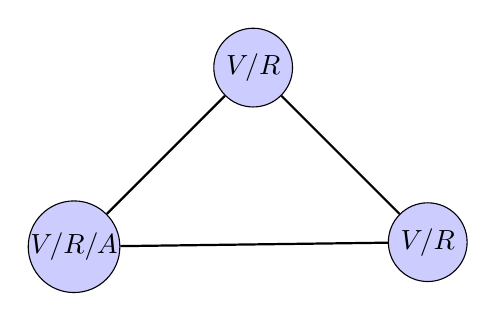
\begin{tikzpicture}
    \node[main node] (1) {$V/R$};
    \node[main node] (2) [below left = 1.5cm and 1.5cm of 1]  {$V/R/A$};
    \node[main node] (3) [below right = 1.5cm and 1.5cm of 1] {$V/R$};
    

    \path[draw,thick]
    (1) edge node {} (2)
    (2) edge node {} (3)
    (3) edge node {} (1);
    
\end{tikzpicture}

Si la heuristica1 por ejemplo hace el analisis empezando por el nodo de abajo a la izquierda que tiene 3 colores y elige el color Verde o Rojo, vamos a suponer el verde, luego continua con el que esta a su derecha, el algoritmo determina que se debe elegir el color rojo ya que sino habria conflictos. Luego al analizar el nodo superior descubre que no es posible elegir un color ya que los dos generan un conflicto, para efectos de este ejemplo vamos a suponer que elige el verde. El grafo que nos queda es el siguiente:

\tikzset{main node/.style={circle,fill=blue!20,draw,minimum size=1cm,inner sep=0pt},
            }

  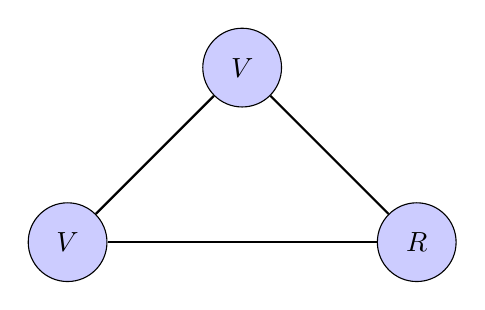
\begin{tikzpicture}
    \node[main node] (1) {$V$};
    \node[main node] (2) [below left = 1.5cm and 1.5cm of 1]  {$V$};
    \node[main node] (3) [below right = 1.5cm and 1.5cm of 1] {$R$};
    

    \path[draw,thick]
    (1) edge node {} (2)
    (2) edge node {} (3)
    (3) edge node {} (1);
    
\end{tikzpicture}

Este grafo tiene un conflito que es resoluble con la busqueda local, ya que al analizar el primer nodo es posible elegir un nuevo color, el Amarillo, lo cual al cambiarlo nos mejoraria nuestro coloreo quedando el siguiente coloreo optimo.

  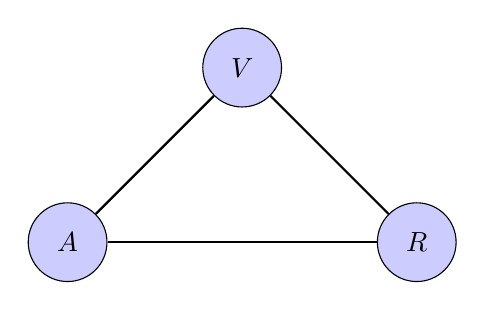
\begin{tikzpicture}
    \node[main node] (1) {$V$};
    \node[main node] (2) [below left = 1.5cm and 1.5cm of 1]  {$A$};
    \node[main node] (3) [below right = 1.5cm and 1.5cm of 1] {$R$};
    

    \path[draw,thick]
    (1) edge node {} (2)
    (2) edge node {} (3)
    (3) edge node {} (1);
    
\end{tikzpicture}\\
\\
Como segundo vecindario tomamos los mismos conflictos que en el primero pero a diferencia del anterior no se trabaja individualmente sobre un solo nodo, sino que se trabaja sobre todos los nodos conflicto que, habiendo cambiado por un color libre, mejoraron la solucion anterior, sobre esto se entrara mas en detalle en la experimentacion(ver secci\'on 4.6).
\subsection{Desarrollo del problema}

\subsection{Pseudo-C\'odigo}

\begin{verbatim}
public Coloreo solve() {
        Listacolores = listaColores()
        ej3.solve() // Se puede elegir cualquier solucion de alguna de las heuristicas
        int [] vectorColores = ej3.getColoreo() //O(Ej3) Con alguna de las heuristicas

        FOR i desde 0 hasta vectorColores.length DO //O(CantColores)
            Color actual = Nuevo Color(vectorColores[i], i) //O(1)
            colores.add(actual); // O(1)
        ENDFOR

        coloreoActual = new Coloreo(grafo, colores) //O(%!!!!%

        IF coloreoActual.esValido() THEN //O(1)
            DEVOLVER coloreoActual
        ELSE
            DEVOLVER resolve(coloreoActual)
        ENDIF
}

private Coloreo resolve(Coloreo colores) {
    int noCambio = 0 //O(1)
    int cantidadSinMejorar = 5 //O(1)
    Coloreo nuevoColoreo //O(1)
    Coloreo mejorColoreo = colores //O(1)

    WHILE !mejorColoreo.esValido() && noCambio < cantidadSinMejorar //O(cotaBruta)
        nuevoColoreo = getProximoColoreo(mejorColoreo) //O(getProximoColoreo)

        IF nuevoColoreo.cantidadDeConflictos() <= mejorColoreo.cantidadDeConflictos() THEN //O(1)
            mejorColoreo = nuevoColoreo; //O(1)

            IF nuevoColoreo.cantidadDeConflictos() == mejorColoreo.cantidadDeConflictos() //O(1) THEN
                noCambio++ //O(1)
            ELSE
                noCambio = 0 //O(1)
            ENDIF
        ELSE
            noCambio = cantidadSinMejorar //O(1)
        ENDIF
    ENDWHILE
    DEVOLVER mejorColoreo
}


CotaBruta: Lo peor que puede suceder es que tengamos un grafo de N nodos tal que este 
pintado del mismo color y tenga N conflictos. Si cada
iteracion, intentamos solucionar 1 conflicto y lo logramos,
podriamos tener N iteraciones hasta llegar a un coloreo valido.\\
\\

Coloreo getProximoColoreo(Coloreo colores)
    Coloreo nuevoColoreo //O(1)
    Coloreo mejorColoreo = colores //O(1)

    FOREACH colores.getConflictos() AS c //O(CantidadConflictos) $\subset$ O(N)
        ArrayList<Color> nuevosColores = new ArrayList<Color>(colores.getColores()); //O(1)
        TreeSet<Integer> coloresOcupados = new TreeSet<Integer>(); //O(1)
        NodoMateria nodoActual = grafo.getMateria(c.getId()); //O(1)


        FOREACH nodoActual.getAdyacentes() AS vecino //O(CantVecinos) $\subset$ O(N)
            List<Color> coloresSeteados = colores.getColores(); //O(1)
            int color = coloresSeteados.get( vecino.getId() ).getColor(); //O(1)
            coloresOcupados.add(color); //O(1)
        ENDFOREACH

        ArrayList<Integer> coloresPosibles = Copia(nodoActual.getColoresPosibles())
        coloresPosibles.removeAll(coloresOcupados)

        IF ! coloresPosibles.isEmpty()
            Color actual = new Color(nodoActual.getId(), coloresPosibles.get(0));
            nuevosColores.set(nodoActual.getId(), actual);
            nuevoColoreo = new Coloreo(grafo, nuevosColores);
            IF nuevoColoreo.cantidadDeConflictos() <= mejorColoreo.cantidadDeConflictos()
                mejorColoreo = nuevoColoreo;
            ENDIF
        ENDIF
    ENDFOREACH

    DEVOLVER mejorColoreo
}

Como nueva vencindad se probo lo siguiente:

public Coloreo solveVecindad2() {
    Listacolores = listaColores()
    ej3.solve() // Se puede elegir cualquier solucion de alguna de las heuristicas
    int [] vectorColores = ej3.getColoreo() //O(Ej3) Con alguna de las heuristicas

    FOR i desde 0 hasta vectorColores.length DO //O(CantColores)
        Color actual = Nuevo Color(vectorColores[i], i) //O(1)
        colores.add(actual); // O(1)
    ENDFOR

    coloreoActual = new Coloreo(grafo, colores) //O(%!!!!%

    IF coloreoActual.esValido() THEN //O(1)
        DEVOLVER coloreoActual
    ELSE
        DEVOLVER resolveVecindad2(coloreoActual)
    ENDIF
}

private Coloreo resolveVecindario2(Coloreo colores) {
    int noCambio = 0 //O(1)
    int cantidadSinMejorar = 5 //O(1)
    Coloreo nuevoColoreo //O(1)
    Coloreo mejorColoreo = colores //O(1)

    WHILE !mejorColoreo.esValido() && noCambio < cantidadSinMejorar //O(cotaBruta)
        nuevoColoreo = getProximoColoreoVecindario2(mejorColoreo) //O(getProximoColoreo)

        IF nuevoColoreo.cantidadDeConflictos() <= mejorColoreo.cantidadDeConflictos() THEN //O(1)
            mejorColoreo = nuevoColoreo; //O(1)

            IF nuevoColoreo.cantidadDeConflictos() == mejorColoreo.cantidadDeConflictos() //O(1) THEN
                noCambio++ //O(1)
            ELSE
                noCambio = 0 //O(1)
            ENDIF
        ELSE
            noCambio = cantidadSinMejorar //O(1)
        ENDIF
    ENDWHILE
    DEVOLVER mejorColoreo
}

Coloreo getProximoColoreoVecindario2(Coloreo colores)
    Coloreo nuevoColoreo //O(1)
    Coloreo mejorColoreo = colores //O(1)

    FOREACH colores.getConflictos() AS c //O(CantidadConflictos) $\subset$ O(N)
        ArrayList<Color> nuevosColores = new ArrayList<Color>(mejorColoreo.getColores()); //O(1)
        TreeSet<Integer> coloresOcupados = new TreeSet<Integer>(); //O(1)
        NodoMateria nodoActual = grafo.getMateria(c.getId()); //O(1)


        FOREACH nodoActual.getAdyacentes() AS vecino //O(CantVecinos) $\subset$ O(N)
            List<Color> coloresSeteados = colores.getColores(); //O(1)
            int color = coloresSeteados.get( vecino.getId() ).getColor(); //O(1)
            coloresOcupados.add(color); //O(1)
        ENDFOREACH

        ArrayList<Integer> coloresPosibles = Copia(nodoActual.getColoresPosibles())
        coloresPosibles.removeAll(coloresOcupados)

        IF ! coloresPosibles.isEmpty()
            Color actual = new Color(nodoActual.getId(), coloresPosibles.get(0));
            nuevosColores.set(nodoActual.getId(), actual);
            nuevoColoreo = new Coloreo(grafo, nuevosColores);
            IF nuevoColoreo.cantidadDeConflictos() <= mejorColoreo.cantidadDeConflictos()
                mejorColoreo = nuevoColoreo;
            ENDIF
        ENDIF
    ENDFOREACH

    DEVOLVER mejorColoreo
}

\end{verbatim}

\subsection{Justificaci\'on y Complejidad}
Para comenzar, tendremos la complejidad de llamar a la heuristica del primer ejercicio para poder comenzar la busqueda. Luego de esos sumaremos el costo de que para cada conflicto que tengamos (que esta acotado por N), querremos revisar todos nuestros colores y todos los colores de todos nuestros vecinos para ver si tenemos un color disponible para solucionar el conflicto. Nuestros colores estan acotados por la cantidad maxima de colores que tenga un nodo (que llamaremos MaxCantColores) y la cantidad de vecinos estan acotadas por la cantidad de nodos del grafo. Por ende la complejidad quedaria  O(EJ3+N^2 * MaxCantColores).\\

\subsection{Tests y Performance}

Lo que vamos a testear en esta parte sera ver como se comportan la heuristica de busqueda local para grafos de gran cantidad de nodos pero poco densos, separando los casos donde tenemos muchos y pocos colores. 

Para ver los conflictos en 10 colores tenemos que:
\pagebreak

\begin{figure}[h!]
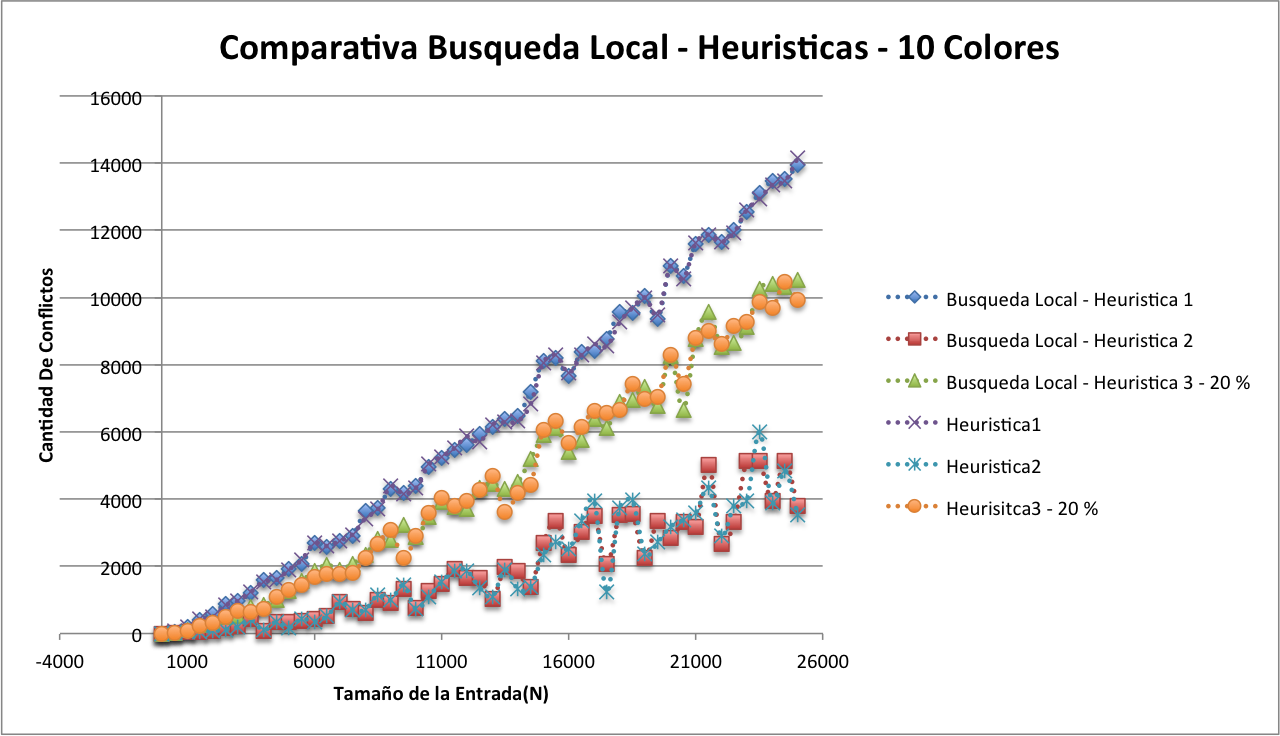
\includegraphics[width=140mm]{ejercicio4/ej4-comparativa-local-heuristicas.png}
\centering
\caption{Comparacion conflictos por heuristica-10 colores}
\label{overflow3}
\end{figure}
Como podiamos imaginar, no existe coloreo valido y vemos que la calidad de nuestro resultado depende mas que nada de la calidad con la cual elegimos nuestra heuristica de arranque. Uno podria suponer que mientras mejor es nuestra subsolucion por donde arrancamos, mejor sera nuestra nuestra solucion final. Sin embargo todavia no sabemos que sucede con la cantidad de iteraciones. Una hipotesis que tenemos es que si arracas con una peor subsolucion, el algortimo tendra la chance de mejorar mayor cantidad de veces y llegar a una mejor solucion que empezando de una buena subsolucion e iterando pocas veces. Luego lo analizaremos para una cantidad de colores mas interesante.\\  

Para analizar el tiempo de ejecucion tenemos que:
\begin{figure}[h!]
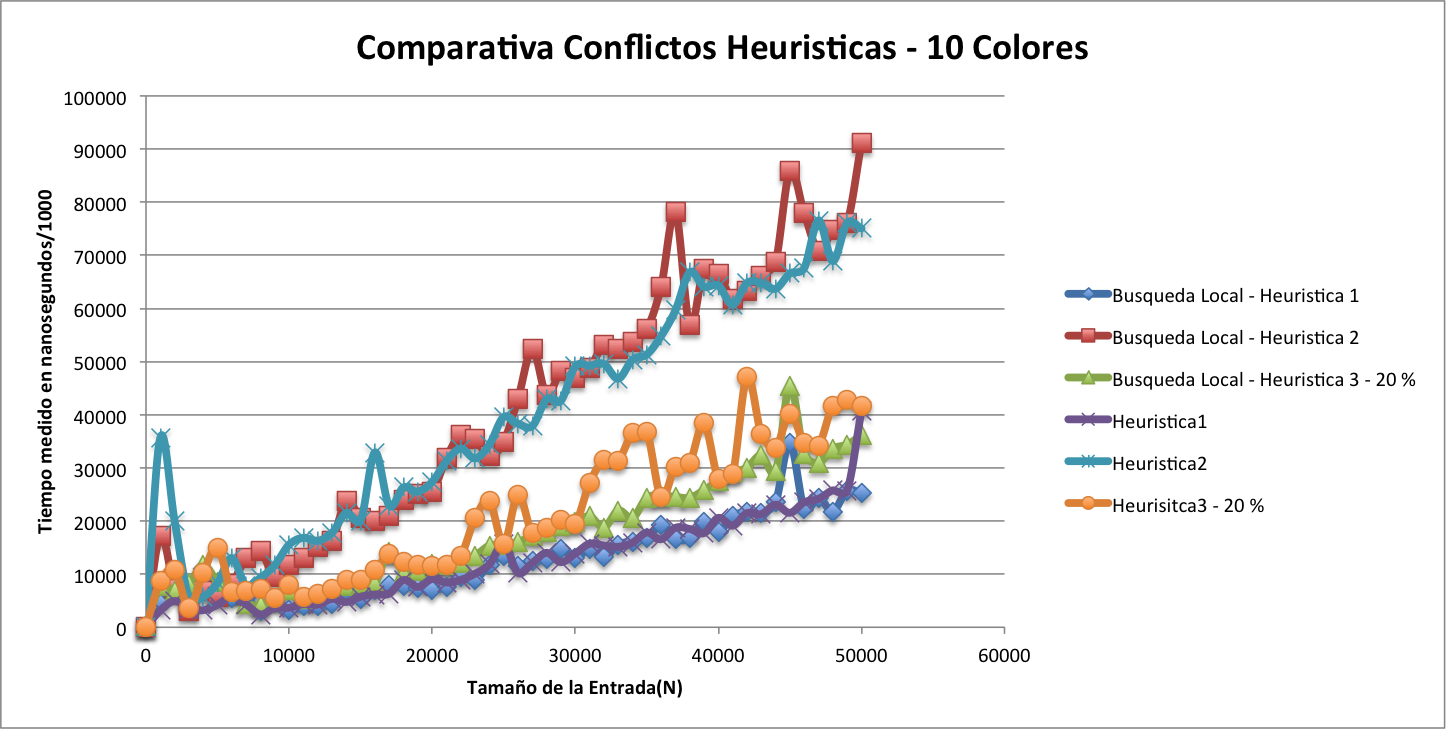
\includegraphics[width=140mm]{ejercicio4/ej4-comparativa-local-heuristicas-10.png}
\centering
\caption{Comparacion Best Vs Worst}
\label{overflow3}
\end{figure}
\pagebreak
La informacion que nos da este grafo es que basicamente el tiempo de ejecucion depende tambien mucho de la heuristica que elijamos al principio. No solo eso sino que nos muestra que nuestra busqueda local nunca podra estar por debajo de la golosa en relacion al tiempo. Ademas el grafico nos muestra que la segunda parte de la suma en en analisis de complejidad (n^2 *MaxCantColores) no es muy relevante y no aporta demasiado al tiempo de ejecucion.\\

Antes de analizar los casos para 500 colores, es trivial que alcanzan para colorear un grafo poco denso de menos de 26k nodos (mayor escala con la cual analizamos el tiempo de ejecucion para 10 colores),\\
Por lotro lado
\begin{figure}[h!]
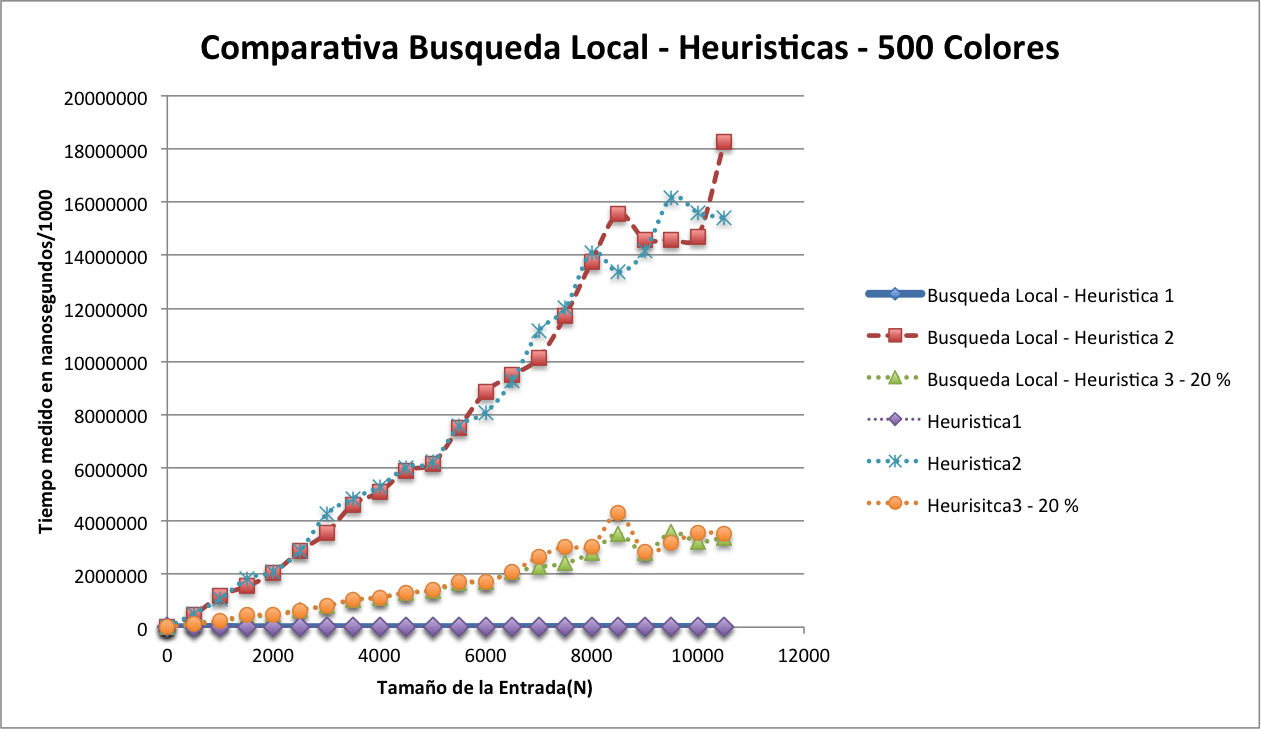
\includegraphics[width=140mm]{ejercicio4/ej4-comparativa-local-heuristicas-500.png}
\centering
\caption{Comparacion Best Vs Worst}
\label{overflow3}
\end{figure}

Para mostrar que realmente la B\'usqueda Local pod\'ia resolver varios conflictos en un grafo, decidimos generar instancias con coloreos muy conflictivos y tratar de mejorarlas con nuestra heur\'istica.
Tomamos grafos de N nodos y los pintamos a todos del mismo color, esto nos crea la mayor cantidad de conflictos posibles para cada uno, variando seg\'un sus conexiones. Luego aplicamos nuestra B\'usqueda local y obtenemos los siguientes resultados

\begin{figure}[h!]
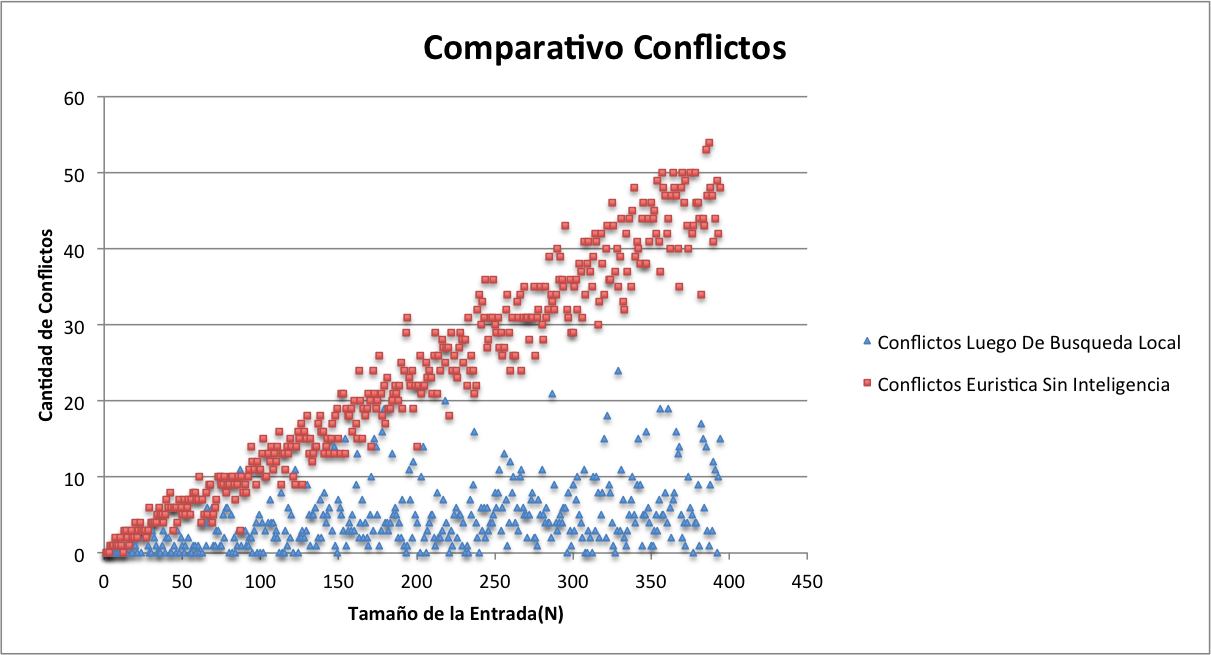
\includegraphics[width=140mm]{ejercicio4/ej4-conflicto}
\centering
\caption{Conflictos reducidos luego de utilizar b\'usqueda lineal.}
\label{overflow3}
\end{figure}
ej4-conflicto

Podemos ver que efectivamente logramos reducir la cantidad de conflictos en gran medida y al ser una b\'usqueda determin\'istica concluimos con que no podr\'iamos encontrar una mejor soluci\'on por este medio. \\

%prueba con una nueva vecindad

Hasta el momento para encontrar alguna modificacion lo que se hacia era probar resolver todos los conflictos individualmente y ver cual mejoro mas la solucion. Como segunda vecindad se intento probar que pasaba si se modificaban todos los nodos al mismo tiempo, esto es si modificar un conflicto redujo los mismos entonces cuando se quiera arreglar el proximo conflicto que tome como base la instancia mejorada previamente.

Para comparar las vecindades se corrierio una instancia del ejercicio3 y sobre esta se corrio el vecindario 1 y 2 por separado y la cantidad de conflictos totales al final de estos fue la siguiente.

\begin{figure}[h!]
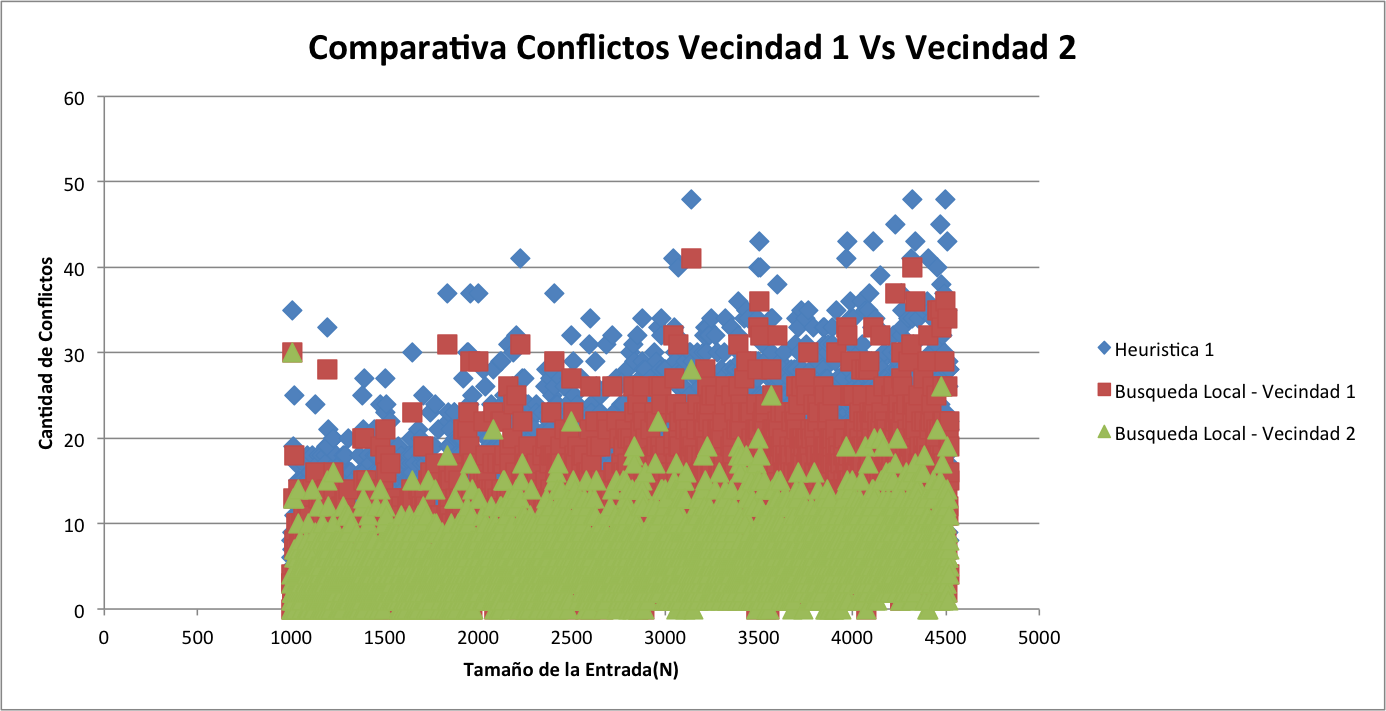
\includegraphics[width=140mm]{ejercicio4/ej4-comparativa-vecindades}
\centering
\caption{Comparaci\'on conflictos ej3 vs vecindarios}
\label{overflow3}
\end{figure}

Se puede observar que arreegla muchos mas conflictos el vecindario 2. Nuestra hipotesis es que al modificar alg\'un conflicto se saca un color de un nodo y se pone otro, esto libera un color y da la posibilidad de que pueda ser utilizado por los nodos vecinos a este y, si el conflicto siguiente es adyacente puede tener la posibilidad de elegir un color diferente a los que podia anteriormente, para algunos casos del vecindario 1 que no tenian mas solucion, este puede dar nuevas posibilidades a los conflictos que esten trabados a poder elegir un color mas.

\pagebreak


